\documentclass[a4paper,12pt]{report}
\usepackage[utf8]{inputenc}
\usepackage{graphicx}
\usepackage{hyperref}
\usepackage{textcomp}
\usepackage{mathtools}

\begin{document}
\begin{titlepage}
\begin{center}
    \vspace*{1cm}
    
    \Huge
    \textbf{Computer Music Languages and Systems}
    
    \vspace{0.5cm}
    \LARGE
    Homework n° 3\\
   	FM synthesis

    \vspace{1 cm}
    
    \textbf{10574752}
    
    \vspace{0.5cm}
    
    \textbf{10751438}
     
    \vspace{0.5cm}
    
    \textbf{10612929}
     
    
    \vspace{0.5cm}
    
    \textbf{10486570}
    
    \vspace{0.5cm}
    
    \vfill
  
   
    \date{May 2021}
    \vspace{0.3cm}
    \textbf{Master of Science in Music and Acoustic Engineering}
    
    \vspace{0.8cm}
    
    
\includegraphics[width=0.5\textwidth]{logo_positivo.png}
    
\end{center}
\end{titlepage}


\abstract{}
Our group worked on \textbf{Assignment 3}: Create an instrument based on FM synthesis and an interface for controlling it. The link containing the source code can be found on GitHub at: \url{https://github.com/EllDy96/CarlGang/tree/Homework3}
\endabstract{}

\chapter{}
\section{SuperCollider}

\subsection*{Synthetizer definition}

\subsection*{MIDI control}

\subsection*{OSC messages}


\section{Interaction design}

Modules and libraries used:
\begin{itemize}
	\item \href{https://nodejs.org/en/}{ Node.js }
	\item \href{https://socket.io/}{ Socket.io }
	\item \href{https://expressjs.com/}{ Express }
	\item \href{https://p5js.org/}{ p5.js }
	\item\href{https://ml5js.org/}{ ml5.js }
	\item \href{https://github.com/colinbdclark/osc.js/}{ osc.js }
\end{itemize}

The synthesizer can be controlled through hand gestures captured from a webcam. For the hand pose recognition, we used a pre-trained ML model from ml5.js (a javascript framework for creative coding built on top of TensorFlow.js), which takes frame by frame the video stream and return the coordinates of 21 points of the hand (this process is GPU intensive, even though the model is lightweight, a system with a dedicated graphic card is advised for best results). 

\begin{figure}[h]
\centering
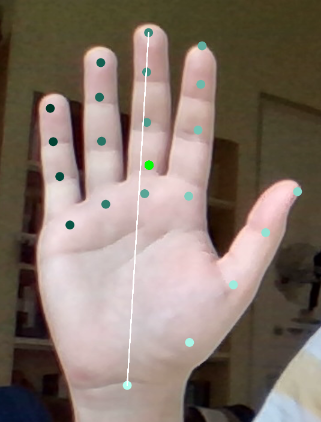
\includegraphics[scale=0.8]{hand.png}
\caption{21 hand points and control parameters}
\end{figure}

From these 21 points (x and y coordinates) we compute 3 parameters:
\begin{itemize}
	\item the centroid (green dot) with coordinates:
	\[x_c = \cfrac{\sum_{i = 1}^{21}x_i}{21}\]
	\[y_c = \cfrac{\sum_{i = 1}^{21}y_i}{21}\]
	\item the distance between the tip of the middle finger $(x_{mf}, y_{mf})$ and the base of the palm $(x_{pb}, y_{pb})$ (length of the white line): 
	\[d = \sqrt{(x_{pb} - x_{mf})^2 + (y_{pb} - y_{mf})^2}\]
	\item the orientation of the hand (the slope of the white line) between $[0, \pi]$:
	\[s = \left\lvert\arctan{\left(\cfrac {y_{mf} - y_{pb}}{x_{mf} - x_{pb}}\right)}\right\rvert \]
\end{itemize}  

 
The user interface is hosted as a web page/application in an Express server, the connection is set up through the framework Socket.io. All the control parameter mentioned above are computed in the client and then sent to the server. From the server, the parameters are written in OSC messages and forwarded to SuperCollider. This last past is handled through the library osc.js, which can generate OSC messages from javascript objects and establish a connection with a receiver (i.e., SuperCollider through an UDP connection). The OSC message has only one path “/params” in which are contained all the parameters as floats.

\begin{figure}[h]
\centering
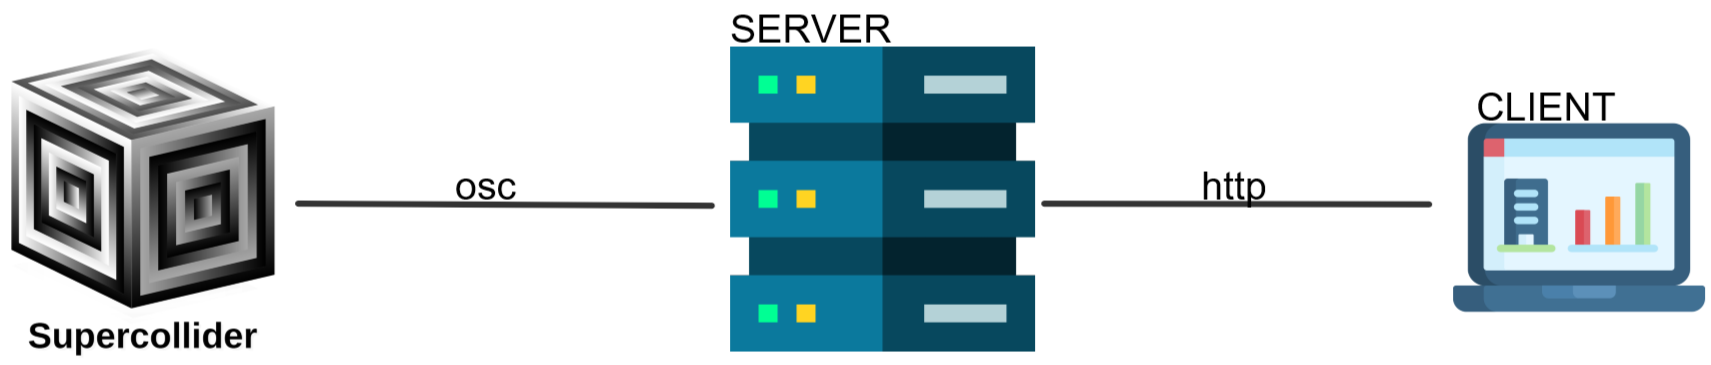
\includegraphics[scale=0.4]{arch.png}
\caption{Application architecture}
\end{figure}


The user interface, as we just said, is a web application in which we imported the libraries ml5.js and p5.js.  We set p5.js in Instance Mode in order to manage 4 different sketches which compose the main window. The bigger p5 sketch at the top left is the one visualizing the webcam, the 21 points of the hand and the control parameters. The other three are a representation of the control parameters using psychedelic animations. At the bottom left we have a visualization for the hand orientation, at the top right for the x and y position of the centroid, and finally at the bottom right, for the distance between the middle finger and the palm base.

\chapter{}
\section{How to use it?}
In order to use the application, run the server using Node.js with the command \verb"node .\server.js". Then connect to the url \verb"localhost:55123" in a browser (it may take some second to load the ML model). Open the synth in SuperCollider and run all the code, it will start to listen for OSC messages through the port 57120. Enjoy!

\section{Improvements roadmap}




\end{document}
